\documentclass{standalone}
\usepackage{tikz}
\usepackage{pgfplots}
\pgfplotsset{width=16cm,height=18cm,compat=1.3}
\pgfplotsset{every tick label/.append style={font=\Huge}}
\usepackage{filecontents}
\usepgfplotslibrary{fillbetween}

\usetikzlibrary{patterns}

\definecolor{citrine}{rgb}{0.89, 0.82, 0.04}
\definecolor{arylideyellow}{rgb}{0.91, 0.84, 0.42}
\definecolor{bronze}{rgb}{0.8, 0.5, 0.2}

\begin{document}
	\centering
		\vspace{1.5em}
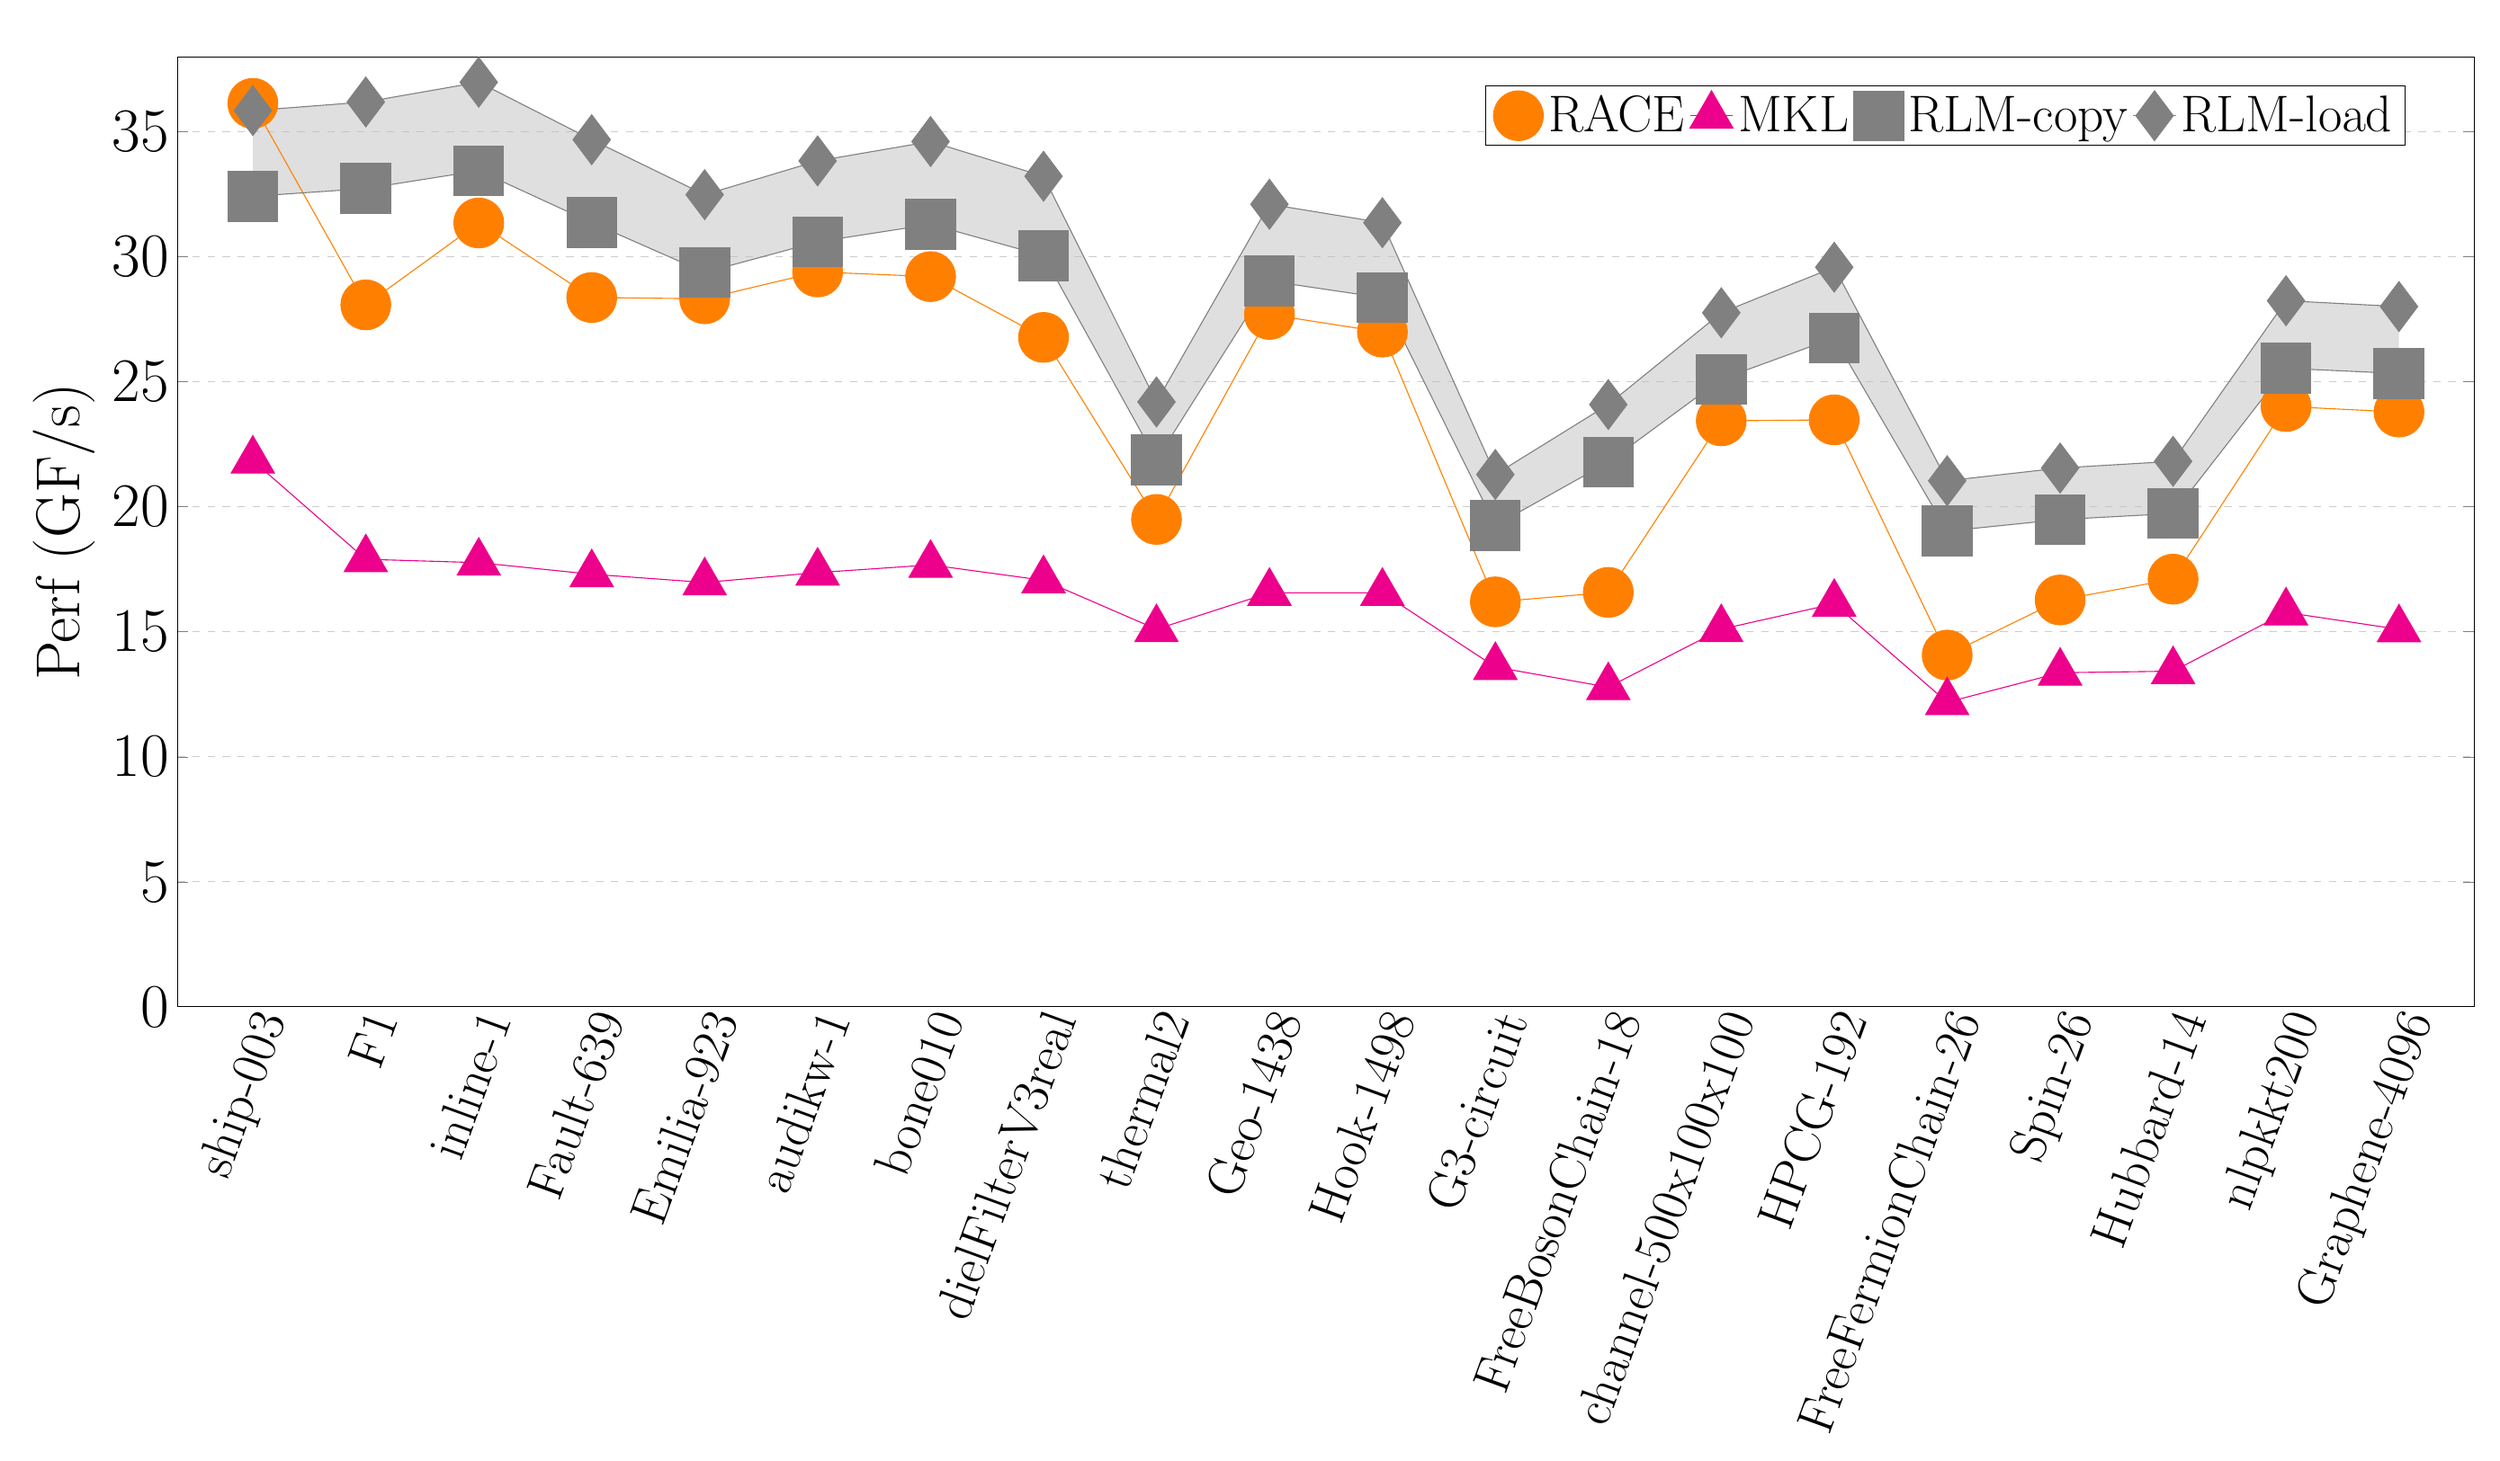
\begin{tikzpicture}
		%	\node at (13.25,15) {\LARGE{}};
			\begin{axis}[
		%	xmin=0.25, xmax=7.25,
			ymin=0, %ymax=3.25,
			ymax=38,
			xtick={1, 2, 3, 4, 5, 6, 7, 8, 9, 10, 11, 12, 13, 14, 15, 16, 17, 18, 19, 20, 21, 22, 23, 24, 25, 26, 27, 28, 29, 30, 31},
		%	ytick={0,0.5,1,1.5,2,2.5,3},
			xticklabels={ ship-003, F1, inline-1, Fault-639, Emilia-923, audikw-1, bone010, dielFilterV3real, thermal2, Geo-1438, Hook-1498, G3-circuit, FreeBosonChain-18, channel-500x100x100, HPCG-192, FreeFermionChain-26, Spin-26, Hubbard-14, nlpkkt200, Graphene-4096},
			width  = 34cm,
			height = 15cm,
			major x tick style = transparent,
			%	minor ytick={1, 5, 10, 15, 20, 25, 30 ,35,40},
			grid = minor,	
			%add_bar_commands
			ymajorgrids = true,
			grid style={dashed, gray!40},
			ylabel = {\Huge{Perf (GF/s)}},
		%	symbolic x coords={Graphene-2048-2048, Graphene-4096-4096, Spin-24-24-24},
			x tick label style={rotate=70, anchor=north east, inner sep=0mm, font={\huge}},
		%	tick label style={font={\Huge}},
			scaled y ticks = false,
			enlarge x limits=0.035,
			legend cell align=left,
			legend style={font=\huge},
			legend columns=-1,
			legend style={
				%at={(1,1.05)},
				%anchor=south east,
				%column sep=1ex,
				legend pos=north east
			},
			%spl_legend_code
			title= {\Huge\scalebox{1.5}{{}}}
			]
\addplot[name path=RACE-SymmSpMV, mark=*, mark size=10pt, mark options={orange}, draw=orange ] plot coordinates{(1,36.140175) (2,28.080251) (3,31.356939) (4,28.372987) (5,28.323231) (6,29.396679) (7,29.210280) (8,26.778583) (9,19.496395) (10,27.696097) (11,26.990050) (12,16.199662) (13,16.577436) (14,23.441453) (15,23.480804) (16,14.069287) (17,16.275497) (18,17.107030) (19,24.014713) (20,23.793009)};
\addplot[name path=MKL-SymmSpMVIE, mark=triangle*, mark size=10pt, mark options={magenta}, draw=magenta] plot coordinates{(1,21.852290) (2,17.902724) (3,17.767401) (4,17.304731) (5,16.975884) (6,17.369550) (7,17.678201) (8,17.062434) (9,15.104626) (10,16.560236) (11,16.560155) (12,13.593018) (13,12.785401) (14,15.105072) (15,16.121380) (16,12.183172) (17,13.365014) (18,13.425972) (19,15.776211) (20,15.101306)};
\addplot[name path=RLM-copy, mark=square*, mark size=10pt, mark options={gray}, draw=gray ] plot coordinates{(1,32.422674442241515) (2,32.73450624945676) (3,33.448600498754566) (4,31.369144841935526) (5,29.379078942831114) (6,30.601322242191323) (7,31.302577971608205) (8,30.046007594627486) (9,21.88158503049584) (10,29.03360063990211) (11,28.36529966442702) (12,19.257114640970986) (13,21.788631100011006) (14,25.107708815137492) (15,26.75615029292358) (16,19.030557606095222) (17,19.49194495374786) (18,19.734157095876782) (19,25.54372630375391) (20,25.33332832179717)};
\addplot[name path=RLM-load, mark=diamond*, mark size=10pt, mark options={gray}, draw=gray ] plot coordinates{(1,35.8519957774786) (2,36.196809795072376) (3,36.98643324381514) (4,34.68703516175563) (5,32.486481523322865) (6,33.83800055626925) (7,34.61342756475907) (8,33.2239507055977) (9,24.195983447182904) (10,32.10446224604561) (11,31.365475590472187) (12,21.293924843381376) (13,24.09319785097371) (14,27.763331862892418) (15,29.586127727752036) (16,21.04340504520145) (17,21.553592977701964) (18,21.821423711786828) (19,28.245466585881726) (20,28.012814971218024)};
\addplot[fill=lightgray,opacity=0.5]
fill between[of= RLM-copy and RLM-load];
	%addplot cmd

	\legend{RACE, MKL, RLM-copy, RLM-load}

	\end{axis}			
\end{tikzpicture}

\end{document}

